\begin{refsection}[operations/tsukamoto/group.bib]
\nocite{*}
\chapter{Facility Operations and Development Team}

\section{Team members}

\begin{itemize}
  \item[] Toshiyuki Tsukamoto (Team Head)
  \item[] Masami Kurokawa (Technical Staff)
  \item[] Mitsuru Tanaka (Technical Staff)
  \item[] Hiroyuki Takitsuka (Technical Staff)
  \item[] Satoru Matsushita (Technical Staff)
  \item[] Katsuyuki Tanaka (Technical Staff)
  \item[] Humio Tsuda (Technical Staff)
  \item[] Mitsuo Iwamoto (Technical Staff)
%  \item[] Hiromi Matsuki (Technical Staff)
%  \item[] Hajime Naemura (Technical Staff)
\end{itemize}

\section{Research Activities}

%Text for research activities.
The K computer facilities have many features not found at other supercomputer sites. These include an expansive and pillar-free computer-room, power supply system that consists of a co-generation system (CGS) and a high-speed current-limiting circuit breaker without uninterruptible power supply (UPS), distribution boards installed not on computer-room walls but under a raised floor, extremely quiet and high-efficiency air conditioners, and water-cooling system for CPUs featuring precise temperature control.
To ensure stable working of K computer and its peripherals, the facility operations and development team (FODT) of the operations and computer technologies division, RIKEN AICS is responsible for operation and enhancement of the facilities. Furthermore, FODT conducts research on the advanced management and operations of AICS’ facilities.
One of the most serious problems is rapid and substantial increase in electricity prices since 2011. Therefore, we investigate the most suitable driving conditions for AICS facilities to achieve effective cost reduction.
Another problem is increased power consumption by AICS. The use of electricity by AICS is strictly limited by a contract between AICS and the local electric supply company. However, recently, the facility’s power consumption exceeded the contract limit. This matter is important because the company requires us to accept a raise in the upper/lower power limit, which amounts to an increase in electricity cost. To prevent this problem, we have investigated a method to control K computer’s power consumption by using emergency job stopping together with the system operations and development team and the software development team of operations and computer technologies division, RIKEN AICS.


\section{Research Results and Achievements}

%Text for research Results and achievements. Journal-artcile~\cite{sample-journal}.
%Conference-paper~\cite{sample-conference}.
%Invited-talk~\cite{sample-invited}.

%For cross referencing, use \verb|\locallabel| and \verb|\localref| to avoid conflicting names defined by other groups. For example, a figure can be referenced as Figure~\localref{fig:sample-label1}.

\subsection{Optimum operation of electric power}

Figure~\localref{fig:fodt-figure1-label} shows the monthly total power supply and the power consumption of K computer from September 2012 to March 2016. The status of power supply, which consists of commercial power purchased from a supply company and the power generated by CGS.

\begin{figure}
\centering
%  \includegraphics[width=0.5\textwidth,keepaspectratio,natwidth=193,natheight=40]
  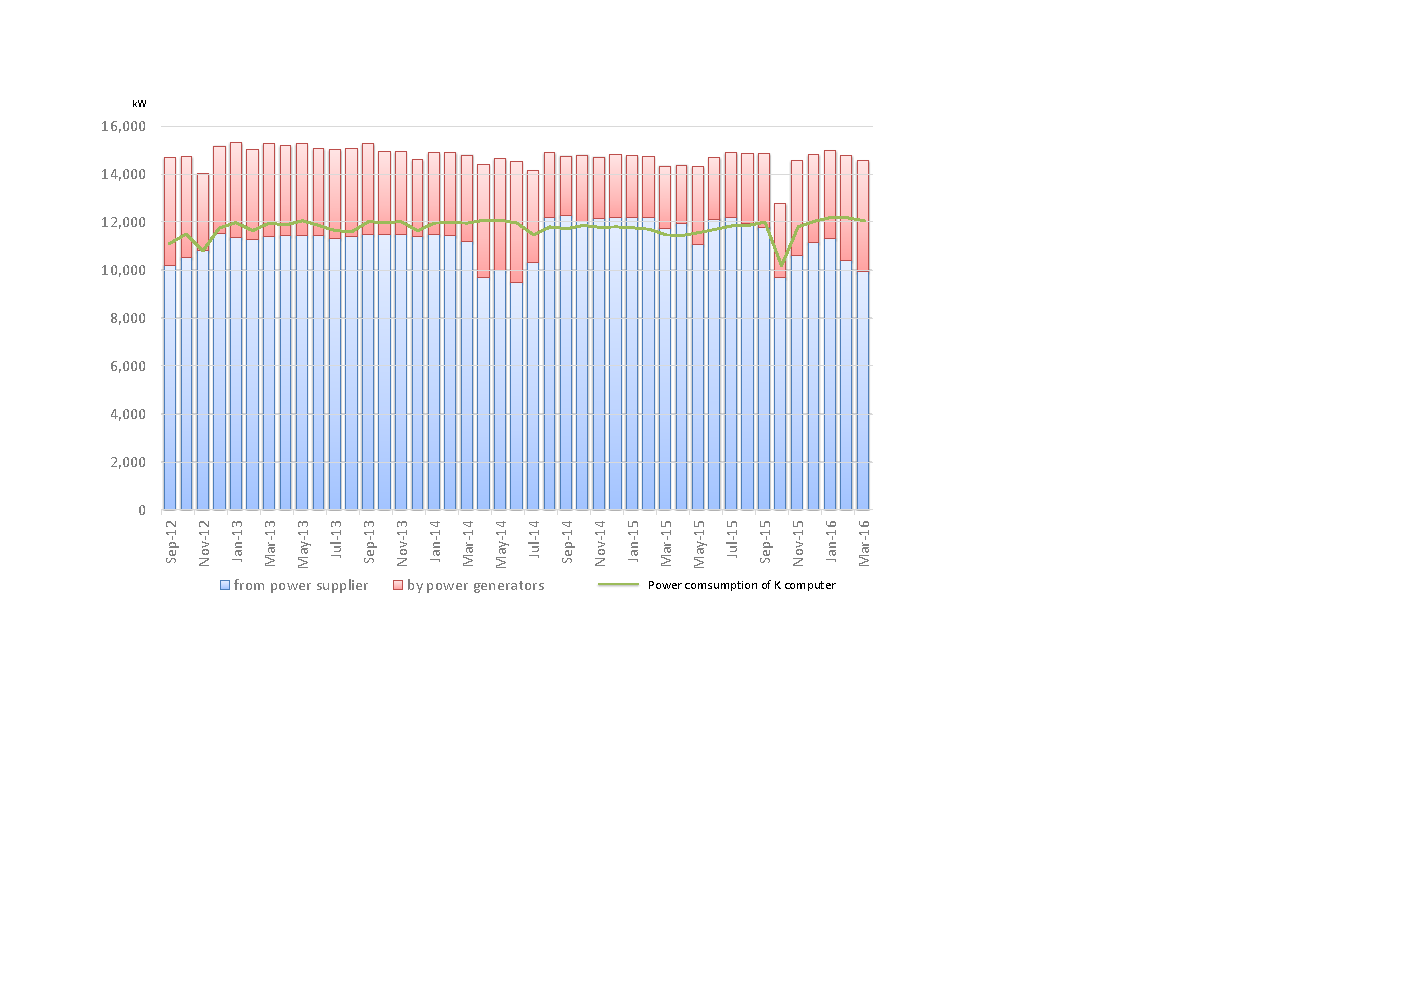
\includegraphics[width=0.9\textwidth,keepaspectratio]
  {operations/tsukamoto/fig/figure1.pdf}
  \caption{Monthly power supply and K computer power consumption}
  \locallabel{fig:fodt-figure1-label}
\end{figure}

The power consumption of AICS is almost synchronized with that of K computer. The power consumption of AICS is nearly 15,000 kW on average, and the power consumption of K computer accounts for approximately 80\% (12,000 kW) of AICS’ total consumption.
As shown in Figure~\localref{fig:fodt-figure1-label}, AICS’ electric power supply consists of commercial and CGS power. There are two CGS systems in AICS, and they are used by turn for two weeks at a time. Therefore, at least one CGS is always in use. Commercial electric power is covenanted at about 12,500 kW, and power consumption was approximately 12,000 kW (annual average), which corresponds to approximately 90\% load factor.
To minimize the cost, we try to optimize the ratio of commercial and CGS electricity.
To investigate the optimized conditions that minimize the sum of electricity and gas cost, we determined the costs of several ratios of commercial electricity to CGS electricity. We also constructed a model to describe energy flow of the electric power supply and cooling system. Then, we performed computer simulation using the model and actual operating data. In near future, we intend to clarify the cost-optimized conditions that contribute toward reducing costs.



\subsection{Improvements to power usage effectiveness (PUE)}

We have continued to work on improvements for the effective use of electricity. PUE is a well known indicator of the effectiveness of electricity use.
 To improve PUE, we have attempted to optimize the operation of the air-conditioning system since FY2013.
Figure~\localref{fig:fodt-figure2-label} indicates a change in the annual average power consumption of K computer (including the peripheral devices) and cooling equipment. After FY2013, the power consumption of K computer has been almost flat at approximately 11800 kW, but the power consumption of the equipment decreased gradually from FY2013 to FY2015. Accordingly, the PUE of AICS improved to 1.356 in FY2015 from 1.447 in FY2012, thus contributing to reduction in electricity cost.

\begin{figure}
\centering
%  \includegraphics[width=0.5\textwidth,keepaspectratio,natwidth=193,natheight=40]
  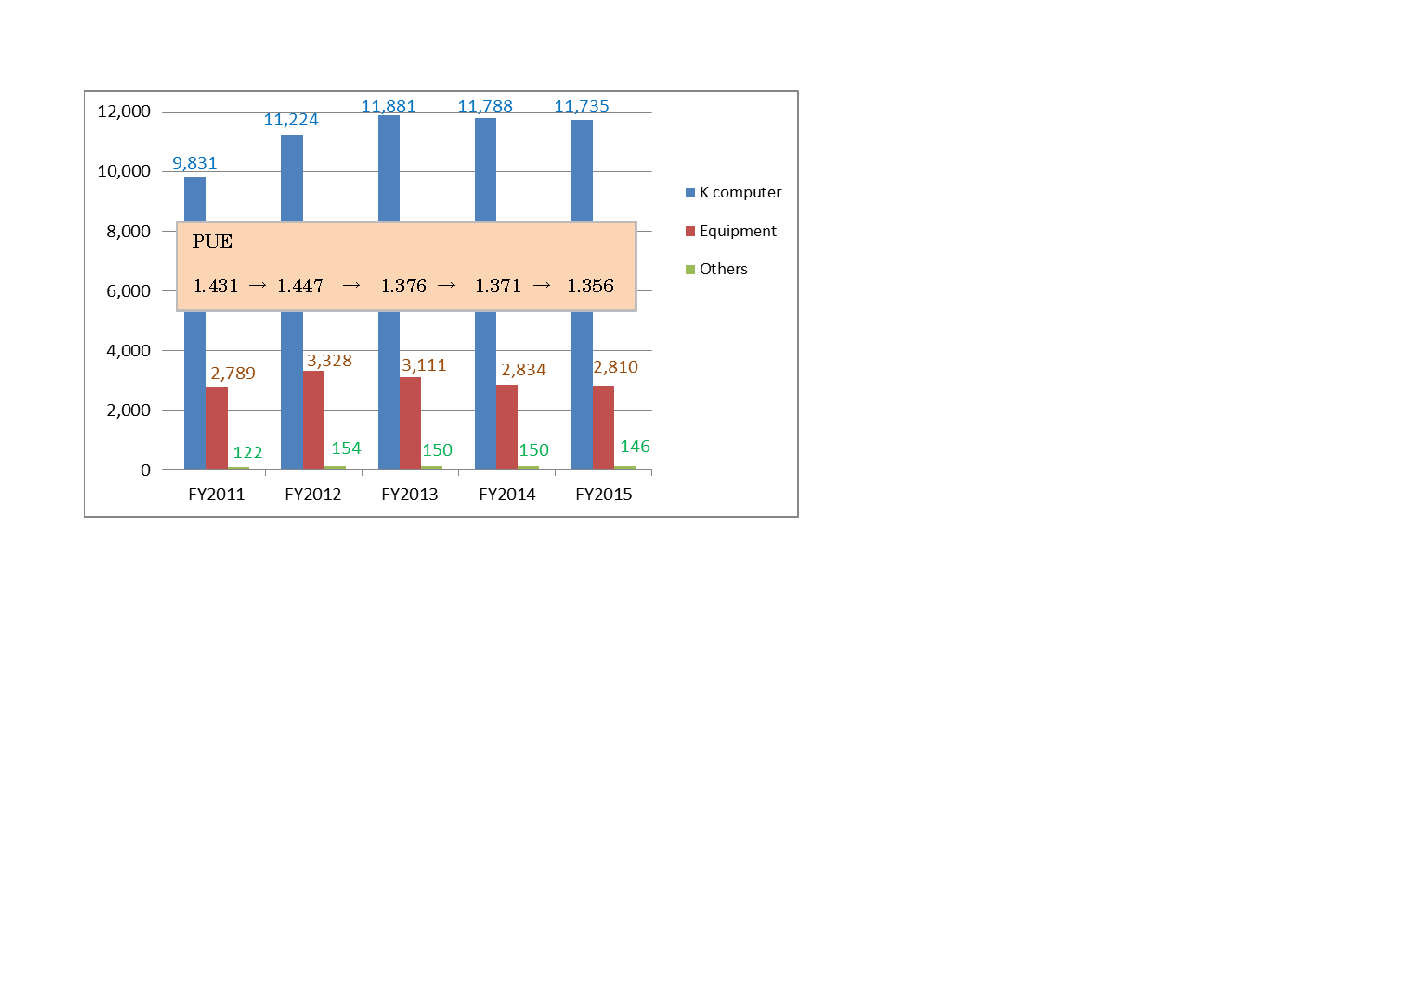
\includegraphics[width=0.9\textwidth,keepaspectratio]
  {operations/tsukamoto/fig/figure2.pdf}
  \caption{Trend in annual average electric power consumption}
  \locallabel{fig:fodt-figure2-label}
\end{figure}

In FY2013, we reduced the electricity cost of air-conditioners by reducing the number of working air-conditioners. Total cooling performance was maintained by lowering the air temperature. We could achieve a reduction of 217 kW in power consumption.
 In FY2014, we focused on the fault-tolerance feature of the air-conditioning equipment. Each air-conditioner has two motors for fault-tolerance. We found that if one of the two motors could be stopped, airflow could be maintained at approximately 60\%. Thus, we reduced power consumption by a further 277 kW in FY2014, and by 24 kW in FY2015.


\section{Schedule and Future Plan}

%Text for schedule and future plan.

We will continue to improve the advanced management and operation of AICS facilities and contribute to the user service of K computer. We will work on reducing costs by investigating and applying the most suitable driving condition to all of the electric power supply and cooling equipment. Furthermore, we will improve electric power control of the entire AICS facility to prevent overshooting the contracted power demand with the system operations and development team.


%%% DO NOT EDIT BELOW

\section{Publications}

%\printbibliography[keyword=journal, heading=subbibliography, title={Journal Articles}, prefixnumbers={1-}, resetnumbers=true]
%\printbibliography[keyword=proceedings, heading=subbibliography, title={Conference Papers}, prefixnumbers={2-}, resetnumbers=true]
%\printbibliography[keyword=invited, heading=subbibliography, title={Invited Talks}, prefixnumbers={3-}, resetnumbers=true]
%\printbibliography[keyword=poster, heading=subbibliography, title={Posters and Presentations}, prefixnumbers={4-}, resetnumbers=true]
%\printbibliography[keyword=deliverable, heading=subbibliography, title={Patents and Deliverables}, prefixnumbers={5-}, resetnumbers=true]

\printbibliography[keyword=journal, heading=subbibliography, title={Journal Articles}, resetnumbers=true]
\printbibliography[keyword=proceedings, heading=subbibliography, title={Conference Papers}]
\printbibliography[keyword=invited, heading=subbibliography, title={Invited Talks}]
\printbibliography[keyword=poster, heading=subbibliography, title={Posters and Presentations}]
\printbibliography[keyword=deliverable, heading=subbibliography, title={Patents and Deliverables}]

\end{refsection}
